% circuit_three_channel_boundary.tex — Three-impedance port at one boundary (Vol 9 Ch.3)
\begin{figure}[htbp]
\centering
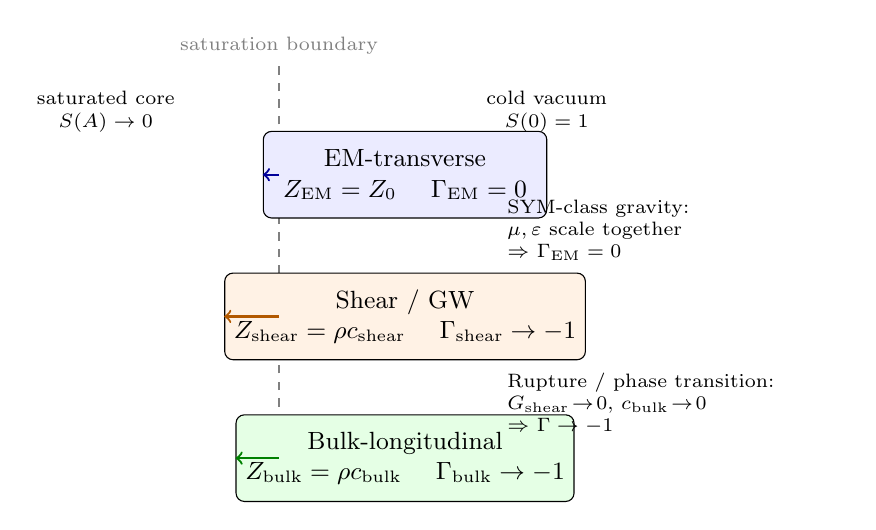
\begin{tikzpicture}[
    port/.style={draw, rounded corners=3pt, minimum width=3.6cm, minimum height=1.1cm, align=center, font=\small},
    line/.style={thick},
    arr/.style={->, thick}
]
    % Boundary plane
    \draw[line, dashed, gray] (0,-2.2) -- (0,3.2) node[above, font=\scriptsize, gray] {saturation boundary};

    % Interior (saturated core)
    \node[font=\scriptsize, align=center] at (-2.2, 2.6) {saturated core\\$S(A)\to 0$};

    % Exterior (cold vacuum)
    \node[font=\scriptsize, align=center] at (3.4, 2.6) {cold vacuum\\$S(0)=1$};

    % Three channel ports
    \node[port, fill=blue!8] (em) at (1.6, 1.8) {EM-transverse\\$Z_{\mathrm{EM}} = Z_0$ \quad $\Gamma_{\mathrm{EM}} = 0$};
    \node[port, fill=orange!10] (sh) at (1.6, 0) {Shear / GW\\$Z_{\mathrm{shear}} = \rho c_{\mathrm{shear}}$ \quad $\Gamma_{\mathrm{shear}} \to -1$};
    \node[port, fill=green!10] (bk) at (1.6, -1.8) {Bulk-longitudinal\\$Z_{\mathrm{bulk}} = \rho c_{\mathrm{bulk}}$ \quad $\Gamma_{\mathrm{bulk}} \to -1$};

    % Arrows from boundary
    \draw[arr, blue!60!black] (0,1.8) -- (em.west);
    \draw[arr, orange!70!black] (0,0) -- (sh.west);
    \draw[arr, green!50!black] (0,-1.8) -- (bk.west);

    % SYM note for EM at gravity boundary
    \node[font=\scriptsize, align=left, text width=4.2cm] at (5.0, 1.1) {SYM-class gravity:\\$\mu,\varepsilon$ scale together\\$\Rightarrow$ $\Gamma_{\mathrm{EM}}=0$};

    % Rupture note for shear/bulk
    \node[font=\scriptsize, align=left, text width=4.2cm] at (5.0, -1.1) {Rupture / phase transition:\\$G_{\mathrm{shear}}\!\to\!0$, $c_{\mathrm{bulk}}\!\to\!0$\\$\Rightarrow$ $\Gamma \to -1$};
\end{tikzpicture}
\caption{Three-channel boundary port (Vol.~9 Ch.~3 \S3; DC impedances Ch.~4). Canonical tables in \S\ref{sec:vol9_device_circuit_models}.}
\label{fig:vol9_circuit_three_channel}
\end{figure}
